% !TEX encoding = UTF-8 Unicode

\documentclass[a4paper, 12pt]{article}

\usepackage[T2A]{fontenc}
\usepackage[utf8x,utf8]{inputenc}
\usepackage[serbian]{babel}
%\usepackage[english,serbianc]{babel}
\usepackage{amssymb}
\usepackage{amsmath}

\usepackage{color}
\usepackage{url}
\usepackage[unicode]{hyperref}
\hypersetup{colorlinks,citecolor=green,filecolor=green,linkcolor=blue,urlcolor=blue}
\usepackage{graphicx}
\graphicspath{ {./slike/} }

\begin{document}

\title{Slobodna bacanja}

\author{Matija Miličević, Jovana Rađenović}

\maketitle

\section{Zadatak}

Košarkaš prilikom slobodnog bacanja izbacuje loptu sa visine koja odgovara 5/4 sopstvene visine. Ako zanemarimo trenje vazduha, i ako je ugao bacanja $\theta$, da bi lopte prošle centrom obruča potrebna je brzina izbačaja $v_\theta$. Sa istom brzinom $v_\theta$ lopta će ući u koš i za bliske uglove $[\theta_1, \theta_2]$ (a da ne dodirne obruč). Za zadatu visinu košarkaša h odrediti onaj ugao bacanja $\theta$ koji obezbeđuje maksimalnu toleranciju $\theta_2 - \theta_1$. Rezultate tabelirati za omiljeni košarkaški klub ili reprezentaciju.

\section{Pojmovi}

Osnovni pojmovi:\\
$h$ - visina košarkaša koji izvodi slobodna bacanja;\\
$h_k$ - visina koša;\\
$\theta$ - ugao izbačaja;\\
$v_\theta$ - brzina izbačaja za ugao $\theta$ pri kojoj lopta prolazi kroz centar obruča;\\
$d_c$ - rastojanje od košarkaša (y-ose) do centra obruča;\\
$r_l$ - poluprečnik lopte;\\
$r_o$ - poluprečnik obruča;\\

%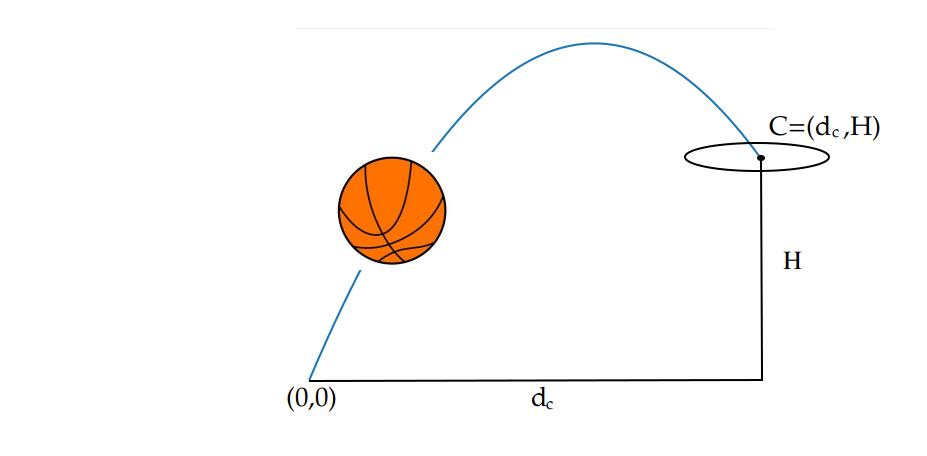
\includegraphics[width=7cm, height=4cm]{pic1} %TODO

\pagebreak


\section{Modeliranje leta lopte} %TODO

Podrazumevaćemo:
\begin{itemize}

\item da je poluprečnik lopte $r_l$ manji od poluprečnika obruča $r_o$:
\[r_l<r_o\] %(3.1.1)

\item da je $\theta$ između $0^0$ i $90^0$:\\
\[0 < \theta < \pi/2\]

\item da je visina koša $h_k$ veća od visine izbačaja košarkaša $\dfrac{_5}{^4}h$:\\
\[h_k > \dfrac{_5}{^4}h\]  %\hfill \centerline{}
%(ovo nije obavezno ali olakšava crtanje slike)\\

\end{itemize}


Posmatraćemo centar lopte kao materijalnu tačku $(x,y)$ koja počinje svoj put iz tačke $(x_0,y_0) = (0,\dfrac{_5}{^4}h)$. Da bi lopta prošla kroz centar obruča u jednom trenutku mora važiti $(x,y) = C$, gde je $C = (d_c,h_k)$.\\

Pošto su visina koša i košarkaša konstantne veličine možemo da transliramo ceo sistem tako da početna tačka centra lopte bude $(x_0,y_0) = (0,0)$, a tačka centra obruča $C = (d_c,h_k-\dfrac{_5}{^4}h)$.
Zbog jednostavnosti zapisa uzećemo da je $H = h_k-\dfrac{_5}{^4}h$, odnosno $C = (d_c,H)$.\\


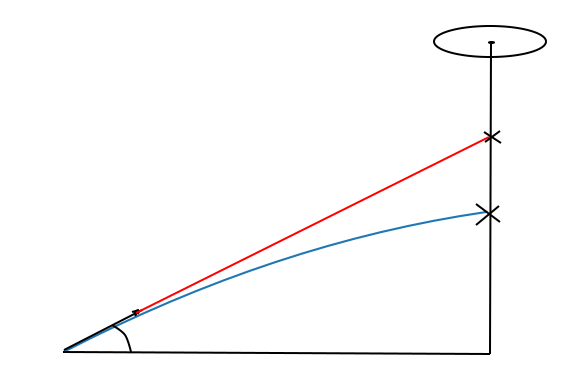
\includegraphics[width=10cm, height=5cm]{pic2} %TODO sredi + naznačiti $y_{max}$)\\

Po ovoj slici možemo primetiti da je polazni problem u stvari jedna vrsta problema kosog hica.

\pagebreak

\subsection{Kretnja lopte}

Možemo da vidimo da na $x$ koordinatu lopte ne utiče nijedna sila (otpor vazduha zanemarujemo), a pošto se lopta kreće brzinom zadatom pri šutu dolazimo da zaključka da važi:\\

\[x(t) = x_0 + v_{\theta x}\cdot t\]

Gde su: $x_0 = 0$; $v_{\theta x} = v_\theta \cdot \cos \theta$; odnosno:

\[x(t) = v_\theta \cdot \cos \theta \cdot t\]

Sa druge strane na $y$ koordinatu sve vreme utiče gravitacija. Uz početnu brzinu zadatu šutom možemo da zaključimo da važi:

\[y(t) = y_0 + v_{\theta y} \cdot t - \dfrac{g \cdot t^2}{2}\]

gde je $g \approx 9.81\dfrac{_m}{^{s^2}}$. Pošto važi da su: $y_0 = 0$; $v_{\theta y} = v_\theta \cdot \sin \theta$; sledi:

\[y(t) = v_{\theta} \cdot \sin \theta\cdot t - \dfrac{g}{2} \cdot t^2\]

Dakle, koordinate centra lopte u svakom trenutku su opisane jednačinama:

\[x(t) = v_\theta \cdot \cos \theta \cdot t\]

\[y(t) = v_{\theta} \cdot \sin \theta \cdot t - \dfrac{g}{2} \cdot t^2\]

\subsection{Odnos brzine i daljine} %TODO izbaciti cdot?

Videli smo da položaj lopte zavisi od parametra vremena $t$. Nas zanima trenutak kada lopta prolazi kroz koš, odnosno $(x,y) = (d_c,H)$. Taj trenutak ćemo obeležiti sa $T$. Sledi:

\[x(T) = v_\theta \cdot \cos \theta \cdot T = d_c\]

\[y(T) = v_{\theta} \cdot \sin \theta \cdot T - \dfrac{g}{2} \cdot T^2 = H\]

\pagebreak

Naš zadatak je da:

\begin{enumerate}
\item Nadjemo za ugao $\theta$ takvo $v_{\theta}$ da lopta prolazi kroz centar obruča
\item Da za to $v_{\theta}$ nadjemo najmanji ($\theta_1$) i najveći ($\theta_2$) ugao za koji lopta i dalje upada u koš
\end{enumerate}

Da bi našli $v_{\theta}$ koristimo prethodne dve jednačine. Iz prve jednačine:

\[T = \dfrac{d_c}{v_\theta \cos \theta} \]

Dakle, vidimo odnos vremena i brzine. Gledamo sad drugu jednačinu:

\[v_{\theta} \sin \theta \cdot T - \dfrac{g}{2} \cdot T^2 = H\]

\[\dfrac{g}{2} \cdot T^2 - v_{\theta} \sin \theta \cdot T - H = 0\]

Iz ovoga dobijamo kvadratnu jednačinu po $T$:

\[T_{1,2} = \dfrac{v_{\theta} \sin \theta \pm \sqrt[]{v_{\theta}^2 \sin^2 \theta - 2 g H}}{g}\]

%Posmatramo putanju lopte kao kvadratnu funkciju po $T$.
%TODO dijagram preseka kv. funkcije i prave y = H
Možemo da vidimo da za vrednosti ${v_{\theta}^2 \sin^2 \theta < 2 g H}$ ne postoji rešenje u skupu realnih brojeva. To znači da lopta nikada neće dostići visinu H i samim tim nećemo postići koš.
U slučaju da važi ${v_{\theta}^2 \sin^2 \theta = 2 g H}$, postoji jedno rešenje $T_1 = T_2 = T$. Ovo nam isto ne odgovara jer ne prebacujemo visinu obruča. Samo ćemo uspeti da dobacimo do centra koša odozdo. Nećemo postići pogodak.

Na kraju dolazimo do konačnog slučaja ${v_{\theta}^2 \sin^2 \theta > 2 g H}$. Dobijamo dva rešenja $T_1$ i $T_2$. Ovo znači da je lopta u letu dosegla visinu H u trenutku $T_1$, dalje stigla do najviše tačke leta i pri padu u trenutku $T_2$ prošla savršeno kroz centar obruča. Pošto nas zanima trenutak prolaska kroz obruč uzimamo veće od dva $T$.

\[T = \dfrac{v_{\theta} \sin \theta + \sqrt[]{v_{\theta}^2 \sin^2 \theta - 2 g H}}{g}\]

Takođe ćemo napomenuti da ubuduće važi uslov ${v_{\theta}^2 \sin^2 \theta > 2 g H}$, tj.

\[{\theta} > \arcsin(\sqrt[]{\dfrac{2 g H}{v_{\theta}^2}}) \]

\pagebreak

Nakon izjednačavanja $T$-ova dobijamo:

\[\dfrac{d_c}{v_\theta \cos \theta} = \dfrac{v_{\theta} \sin \theta + \sqrt[]{v_{\theta}^2 \sin^2 \theta - 2 g H}}{g}\]

Posle sređivanja: %TODO (možemo da kvadriramo jer su sve vrednosti pozitivne)

\[v_\theta = \sqrt[]{\dfrac{g d_c^2}{2 \cos^2 \theta (d_c \tan \theta - H)}}\]

Ovo inače predstavlja brzinu neophodnu da bi lopta pri padu prošla kroz tačku $(d_c,H)$.
Inače tokom sređivanja izraza došli smo do novog uslova $d_c \tan \theta - H > 0$, odnosno:

\[{\theta} > \arctan(\dfrac{H}{d_c}) \]

Što je geometrijski logično jer da ne važi ovaj uslov mi bi ciljali ispod koša i uvek bi prebacili daljinu obruča pre nego što bi stigli na njegovu visinu.

%TODO slika!
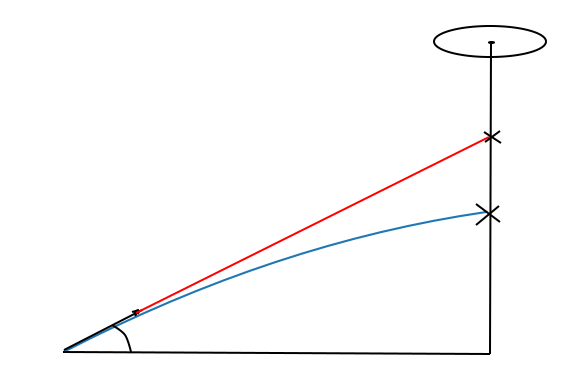
\includegraphics[width=10cm, height=5cm]{pic3}

%TODO broj formule
Iz formule $v_\theta$ još možemo da zaključimo:

\[d = \dfrac{v_\theta \cos \theta}{g}(v_{\theta} \sin \theta + \sqrt[]{v_{\theta}^2 \sin^2 \theta - 2 g H}) \]

Gde smo namerno umesto $d_c$ stavili $d$, jer formula važi za proizvoljnu pozitivnu tačku na x-osi. Sa ove dve formule možemo da odredimo kojom brzinom treba da izbacimo loptu pri uglu $\theta$ da bi ona pala na nivo $H$ posle $d$ pređenog puta. Takođe možemo izračunati koju daljinu će lopta preći pre nego što padne na nivo $H$ ako joj je početna brzina bila $v$.

\pagebreak

\subsection{Uslovi za prolazak lopte kroz obruč} %TODO

Do sada smo loptu posmatrali kao tačku u prostoru (njen centar). Odredili smo dva uslova koja moraju biti ispunjena da bi lopta prošla kroz obruč:

\[{\theta} > \arcsin(\sqrt[]{\dfrac{2 g H}{v_{\theta}^2}}) \]

\[{\theta} > \arctan(\dfrac{H}{d_c}) \]

Pre nego što se pozabavimo traženjem uglova $\theta_1$ i $\theta_2$ moramo da vidimo kada lopta upada u koš.

\[TODO!!!\]

\subsection{Uglovi $\theta_1$ i $\theta_2$} %TODO

Pretpostavimo da $\theta \subseteq (0,\pi/2)$ ispunjava uslove i može se pogoditi koš ako šutiramo pod tim uglom. Postavlja se pitanje kako da odredimo $\theta_1$ i $\theta_2$ za dati ugao $\theta$?

Očigledan način je da u

\[TODO!!!\]



\section{Model rešenja: dvostruka iteracija} %TODO

Jednostavan i očigledan model rešenja je da za svaki mogući ugao $\theta$ nadjemo njihove $\theta_1$ i $\theta_2$ i da kao optimalni ugao izaberemo onaj čija je razlika
$\theta_2 - \theta_1$ maksimalna. Vremenska složenost ovog rešenja je na taj način $O(n \cdot m)$ gde je $n$ broj uglova $\theta$, a $m$ prosek broja uglova $\theta_1$ i $\theta_2$. Naravno pošto uglovi pripadaju neprebrojivom skupu nećemo moći da proverimo rešenje za svaki ugao $\theta$. Moraćemo da diskretizujemo problem time što ćemo odrediti korak iteracije. Manji korak znači veća preciznost, ali i duži rad programa.

\[TODO!!! + KOD!\]

\end{document}